As this usability evaluation study has highlighted, the Monterosa's website gives to users a quite good experience that could be easily improved by solving the found small issues.\\ 
For what concern Navigation, the strength is given by the four landmarks (header (fig. 1), topbar (fig. 2), leftbar (fig. 3) and bottombar (fig. 4)  which:
\begin{itemize}
	\item ensure a consistent aspect between pages;
	\item give an intuitive way to navigate between contents;
	\item overcome all navigation problems related to links' miss between contents of a same topic and structural problems.
\end{itemize}
This aspect could be better managed by adding the possibility to go back to previous page \emph{(for example by including the followed path to reach each page)}; by adding links and letting users to move between similar contents without always accessing the header and by being more consistent in buttons layout and and visibility (for example by always showing only the one related to the selected season).\\Contents have taken the best score between the 3 groups because the website contains lots of information well organized and without visible issues. The only adjustments that could be done is related to adding all missing images and adding some text even in those pages in which there is just an expressive title.\\ Last but not the least, sometimes the layout was found a little too rough but with a small effort could make pages look tidier and more clear (suggestions can be found in section 3.3). The real layout weak point is given by the lack of consistency between the pages reached by clicking over topbar's links,  they should be similar but actually there are 2 main contents' structures (fig. 8 - fig. 9 ). We don't know which one should be used to make it uniform because both have they pros and cons.

\begin{figure}[h!]
	\centering
	\begin{minipage}[b]{0.4\textwidth}
    		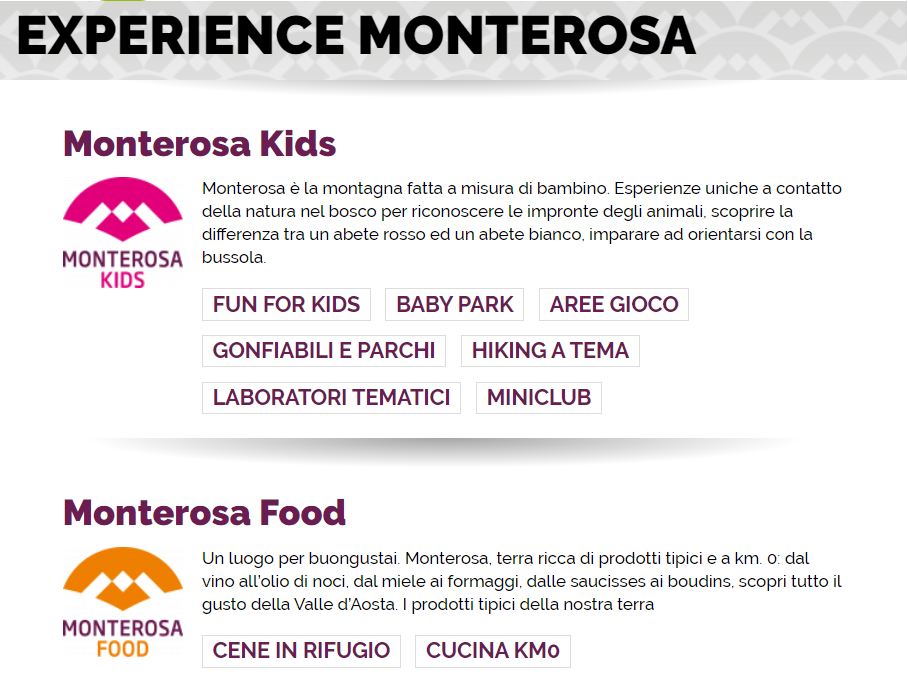
\includegraphics[width=\textwidth]{./assets/structure1.png}
		\caption{Content's structure 1}
	\end{minipage}
	\hfill
	\centering
	\begin{minipage}[b]{0.4\textwidth}
    		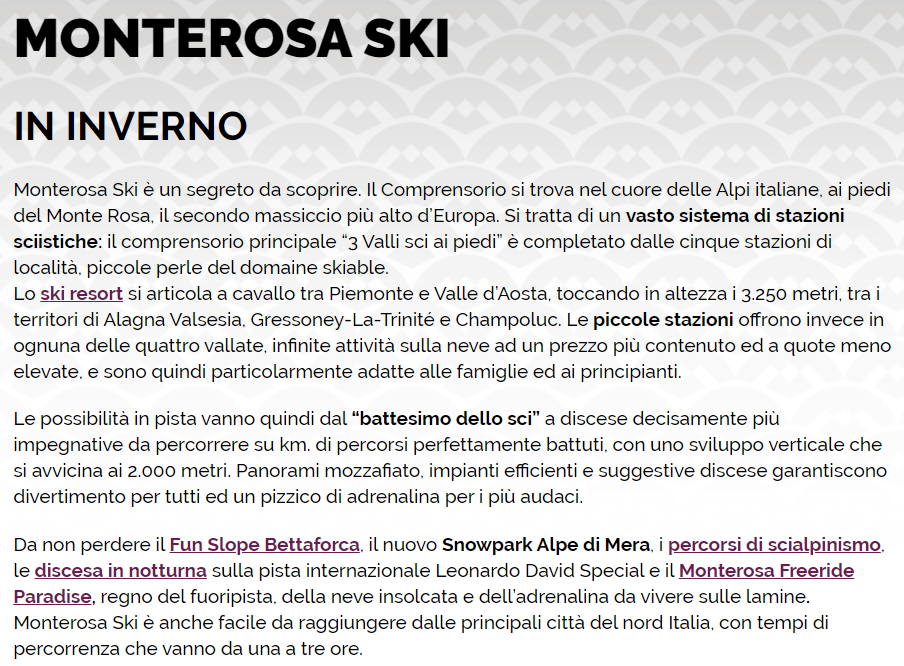
\includegraphics[width=\textwidth]{./assets/structure2.png}
		\caption{Content's structure 2}
	\end{minipage}
\end{figure}
\FloatBarrier

\subsubsection*{Personal Comment}
We encounter some difficulties in alligning our ways of reasoning over the analyzed aspects and also in getting the heuristics limits. We found this project kinda complex but in the same time interesting because it allowed us to understand in a clear way what has an impact over our sentiment as users and how we would like a website to be done.
